\documentclass[11pt]{article}

\usepackage[english]{babel}
\usepackage[utf8]{inputenc}
\usepackage{a4wide}
\usepackage{graphicx}
\usepackage{booktabs}
\usepackage{wrapfig}
\usepackage{subcaption}
\usepackage[margin=1.5cm]{caption}
%\usepackage[framed,numbered]{mcode}
\usepackage{amsmath}
%\usepackage{arevmath}
\usepackage{amssymb}
\usepackage{amsthm}
\usepackage{physics}
\usepackage[version=4]{mhchem}
\usepackage{array}
\usepackage{cases}
\usepackage{pbox}
\usepackage{hepnames}
\usepackage{siunitx}
\usepackage{enumitem}
\usepackage{fancyhdr}
\usepackage{etoolbox}

\patchcmd{\thebibliography}{\section*{\refname}}{}{}{}

\setlength{\parindent}{0.3cm}
\addtolength{\oddsidemargin}{-5mm}
\addtolength{\evensidemargin}{-5mm}
\addtolength{\textwidth}{10mm}
\setlength{\headheight}{14pt}

\pagestyle{fancy}

\begin{document}
	\begin{titlepage}
		\begin{center}
			\hrule
			\vspace*{1cm}
			
			\textbf{\LARGE{Flashlamp Annealing for Improved Ferroelectric Junctions}}\\ 
			\vspace{0.5cm}
			\Large{Master's Degree Project}
			
			\vspace{1.5cm}
			
			\textbf{\Large{Theodor Blom}} \\
			\small{Lund University} \\
			\vspace{0.2cm}
            \small{Project Duration: 12 months, 60 hp}\\
            \vspace{0.2cm}
			\small{\today}
			
			\vfill
			
			\includegraphics[width=0.35\textwidth]{~/Pictures/lu_logo-portrait-en.png}
			
			\vspace{1cm}

            \begin{minipage}{0.51\textwidth}
                \centering
                \textbf{\Large{Mattias Borg}} \\
			    \vspace{0.2cm}
                Division of Nano Electronics,\\
                Department of Electrical and Informations Technology,\\
                Faculty of Engineering, LTH,\\
			    Lund University\\
            \end{minipage}
            \begin{minipage}{0.48\textwidth}
                \centering
                \textbf{\Large{Rainer Timm}} \\
			    \vspace{0.2cm}
                Division of Synchrotron Radiation,\\
                Department of Physics,\\
                Faculty of Science,\\
			    Lund University\\
            \end{minipage}
			\vspace{1cm}
			\hrule
		\end{center}
	\end{titlepage}
\newpage
    \thispagestyle{empty}
    \mbox{}
\newpage
    \tableofcontents
    \begin{abstract}
        Abstract here!
    \end{abstract}
\newpage \pagenumbering{arabic}
    \section{Introduction}
    
    Mål: Introducera området och ge en överblick.\cite{atle2019development}

    \section{Semiconductors and Ferroelectrics}

    Mål: Klargöra varför III-V (utgå från Si) och FE är intressant. Varför gör vi detta? Vad är applikationern? Få med FTJ här!

        \subsection{III-V Semiconductors}

        Mål: Redogör för varför III-V är intressant. Direkt bandgap, lägre DOS --> FTJ

        \subsection{Ferroelectricity}

        Mål: Basics of FE;\ Kristallstrukturer (faser), Polarisation, Domäner och PE-kurvor.

            \subsubsection{\ce{HfZrO2}}

            Mål: Redogör för FE-\ce{HfO2} och beskriv hur \ce{Zr} kommer in i bilden.

        \subsection{Energyband Theory and Leakage Mechanics}

        Mål: Redogör för hur energibanden ser ut med Semiconductor-Insulator-Metal-cap och gå igenom de olika tunnelsätten.

    \section{Fabrication}

    Mål: Redogör för hela processen på LNL.\ 

        \subsection{Processing Methods}

        Mål: Redogör för dem mest intressanta/relevanta metoderna. Kanske bara ALD och FLA?\ 

            \subsubsection{ALD}


            \subsubsection{Flashlamp Annealing}


        \subsection{Sample Fabrication Process}\label{sec:FabProc}

        Mål: Redogör för hela min process.

    \section{Electrical Charcterization}\label{sec:e-char}

    Mål: Redogör för metoderna på E-huset.

        \subsection{PUND and Endurance}\label{sec:PandE}


        \subsection{UniCV}\label{sec:UniCV}
        Frågor att besvara: 
        \begin{itemize}
            \item Hur funkar metoden? 
            \item Vilka defekter ser vi med denna metod? 
        \end{itemize}

    \section{Results and Analysis}
    \iffalse{}
    Mål: Presentera serierna i en rimlig ordning och dra slutsatser från varje serie.

    Tre steg:
    \begin{enumerate}
        \item FlashInt och Temperatur
        \item FlashNum vid olika FlashInt
        \item Förkristallisering för att minska Tpeak (270C och seedlayer)
    \end{enumerate}

    Fokus på frågeställingar!
    \begin{itemize}
        \item Utforska möjligheten kring FLA
        \item Hur bra devices kan vi göra? PUND och Endurance
        \item Fokus på interface defects genom CV!\  
    \end{itemize}
    \fi

    \subsection{Flashlamp Intensity and Film Temperature}
    Crystalization of the hafnia films using the flash lamp annealing (FLA) technique does not immediately reveal the temperature achieved in the films. Due to the short time frames and the geometry of the FLA setup, one must simulate the achieved temperature in the film from the compositional structure of the samples and the measured peak backside temperature during annealing. Furthermore, the experiment parameters of preheating temperature and flash duration are crucial for the simulations and are throughout this work set to \SI{250}{\celsius} and \SI{5}{\milli\second} respectively. Figure~\ref{fig:res_ComsolSim} shows the resulting film temperature depending on flash intensity with the choosen set parameters.
    
    \begin{figure}[ht!]
        \centering
        \includegraphics[width=.40\textwidth]{~/Pictures/image-placeholder-500.jpg}
        \caption{Figure showing how flashintensity relates to the peaktemperarure of the films through simulations. From this figure onwards we can then stick to Peak Temperature instead of Flash Intensity.}\label{fig:res_ComsolSim}
    \end{figure}

    Explain in detail the figure above here and conclude the subsection. What type of figure (s) can I expect here??

    \subsection{Sample Specifications and Characterization}
    In addition to the samples of focus in this work, samples were processed using RTP as the annealing method in paralell with FLA samples. These samples proves as a point of comparison for the characterization of the FLA samples throughout the work. The RTP samples were annealed at a temperature of \SI{600}{\celsius} for 30 seconds. Through the electrical characterization described in Section~\ref{sec:PandE} the remnant polarization ($P_r$), coercive field ($E_c$) and endurance were measured and tabulated in table~\ref{tab:RTPref}.

    \begin{table}[ht!]
        \centering
        \caption{Electrical characteristics for the RTP reference samples measured using a cycling voltage of \SI{3}{\volt}.}\label{tab:RTPref}
        \begin{tabular}{rlrl}
            \toprule
            \multicolumn{4}{c}{PUND and Endurance}\\\midrule
            Remnant Polarization & $P_r$ & $29.03 \pm 0.21$ & \si{\micro\coulomb/\centi\meter^2}\\
            Coercive Field & $E_c$ & $1.23 \pm 0.18$ & \si{\mega\volt/\centi\meter}\\
            Endurance & & $0.23 \pm 0.11$ & $10^5$ cycles\\\bottomrule
            %Defect Density & $D_d$ & $10.0 \pm 1.0$ & $10^{12}$\si{/cm^2} \\
        \end{tabular}
    \end{table}

    The processing of the FLA samples are outlined in Section~\ref{sec:FabProc}. For the first FLA series, hereby denoted sample series 1, the flash intensity was varied between 15-\SI{32.5}{\joule/\centi\meter^2} to reach different peak temperatures in the film. The film deposition and annealing conditions for these samples are summarized in table~\ref{tab:FlashIntC}.

    \begin{table}[ht!]
        \centering
        \caption{Selected processing conditions for sample series 1.}\label{tab:FlashIntC}
        \begin{tabular}{rlccccc}
            \toprule
            \multicolumn{2}{l}{Sample Number} & 1 & 2 & 3 & 4 & 5 \\\midrule
            \multicolumn{1}{c}{HZO} & & & & & & \\
            Growth Temperature & [\si{\celsius}] & 200 & 200 & 200 & 200 & 200 \\
            Film Thickness & [\si{\nano\meter}] & 10 & 10 & 10 & 10 & 10 \\\midrule
            \multicolumn{1}{c}{FLA} & & & & & & \\
            Preheat Temperature & [\si{\celsius}] & 250 & 250 & 250 & 250 & 250 \\
            Flash Intensity & [\si{\joule/\centi\meter^2}] & \textbf{15} & \textbf{20} & \textbf{25} & \textbf{30} & \textbf{32.5} \\
            Number of Flashes & & 1 & 1 & 1 & 1 & 1 \\\bottomrule
        \end{tabular}
    \end{table}

    Resulting electrical characterization from sample series 1 are shown in figure~\ref{fig:res_FlashIntC}. Samples annealed with an intensity less than \SI{25}{\joule/\centi\meter^2} did not show any ferroelectric behaviour and are hence omitted from some of the figures. As shown in figure~\ref{fig:res_FlashIntC}a and b the PUND characteristics show ferroelectric behaviour with a strong dependance on peak film temperature. However, for higher peak temperatures these characteristics decline to both weaker polarization response and higher coercive fields which is undesireable. The peak PUND performance at \SI{30}{\joule/\centi\meter^2} does not reach the characteristics of the RTP references outlined in table~\ref{tab:RTPref} which shows that the energy deposited during the annealing process is not enough to crystalize the entire HZO film while not inducing other effects to reduce the ferroelectric response.\\

    Although reduced PUND characteristics were found for these samples, figure~\ref{fig:res_FlashIntC}c show an increased endurance for the flash annealed samples compared to the RTP reference.

    \begin{figure}[ht!]
        \centering
        (a)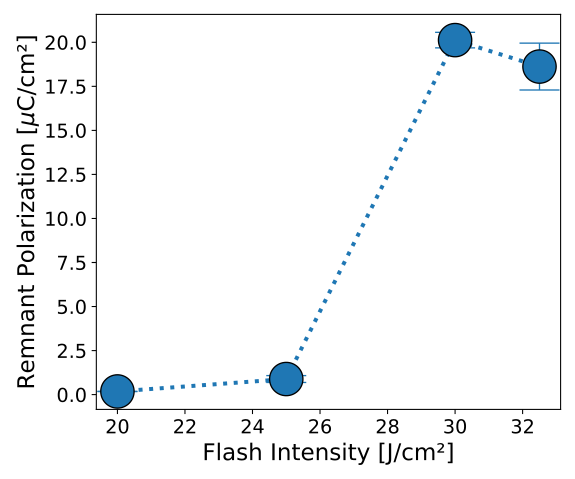
\includegraphics[width=.45\textwidth]{../Fig/FlashIntC_PrTrends.png}
        (b)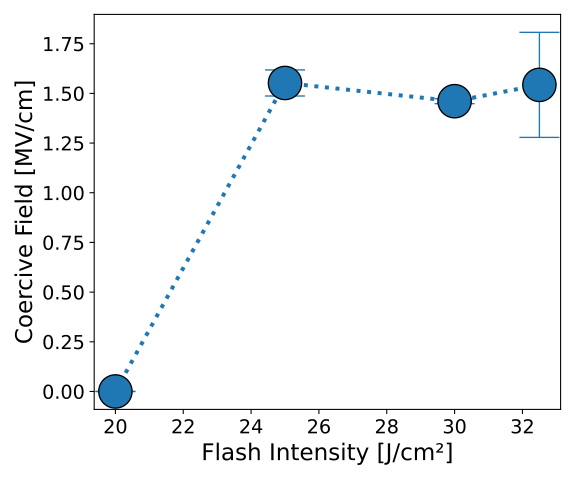
\includegraphics[width=.45\textwidth]{../Fig/FlashIntC_EcTrends.png}
        (c)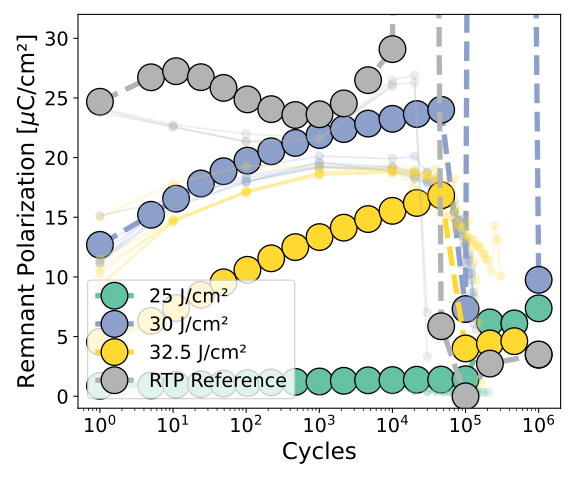
\includegraphics[width=.45\textwidth]{../Fig/FlashIntC_EnduTrends.png}
        (d)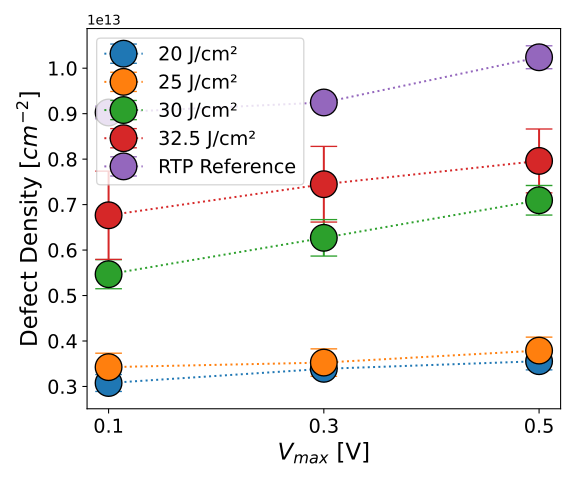
\includegraphics[width=.45\textwidth]{../Fig/FlashIntC_DDTrends.png}
        \caption{Figure showing all measured data from an intensity-varied batch. Low-doped subtrate, 200C ALD, HZO 1:1, 250C preheat, 5ms flash. RTP reference is included for Endurance and Defect Density.}\label{fig:res_FlashIntC}
    \end{figure}

    \begin{figure}[ht!]
        \centering
        (a)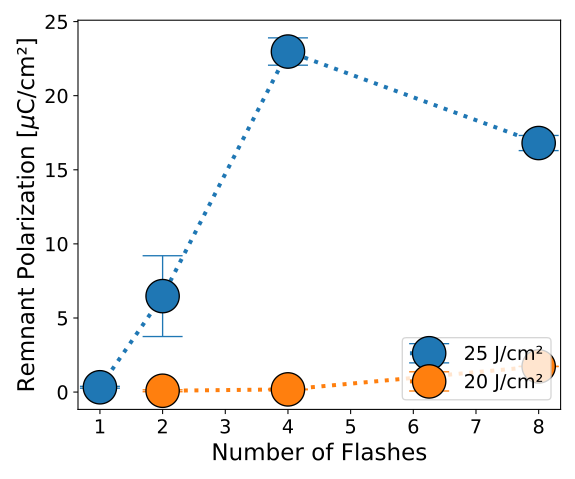
\includegraphics[width=.45\textwidth]{../Fig/FlashNumA+C_PrTrends.png}
        (b)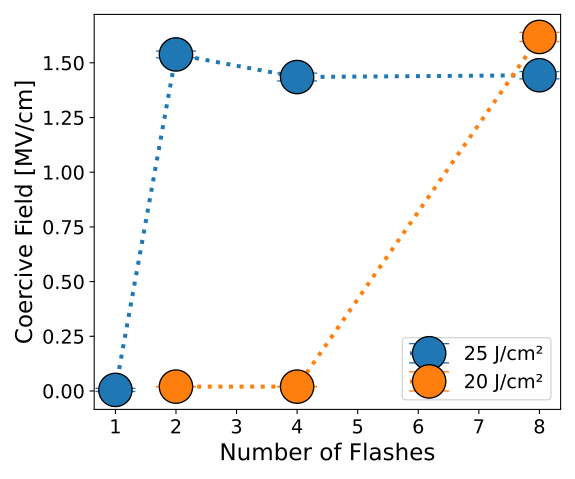
\includegraphics[width=.45\textwidth]{../Fig/FlashNumA+C_EcTrends.png}
        \caption{Figure showing Pr and Ec trends from flashnumber-varied batches. Low-doped subtrate, 200C ALD, HZO 1:1, 250C preheat, 5ms flash at $\SI{25}{\joule/\centi\meter^2}$ and \SI{20}{\joule/\centi\meter^2}.}\label{fig:res_FlashNumAC_PrEc}
    \end{figure}

    \begin{figure}[ht!]
        \centering
        (a)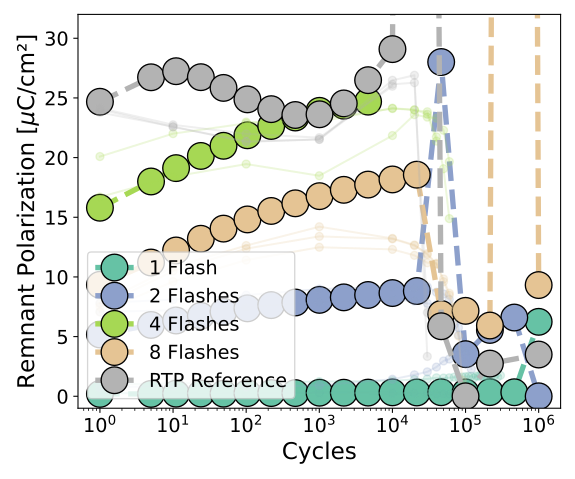
\includegraphics[width=.45\textwidth]{../Fig/FlashNumA_EnduTrends.png}
        (b)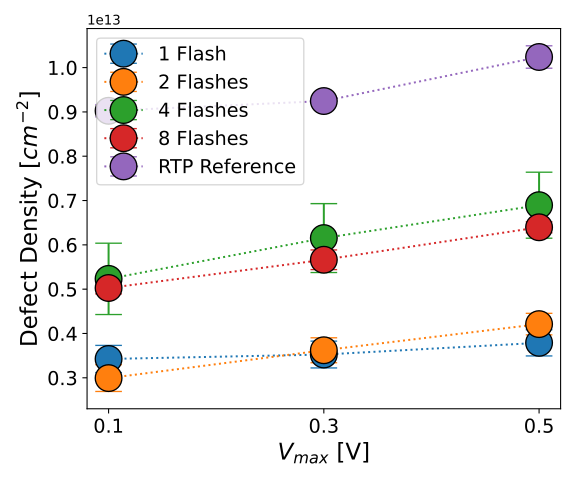
\includegraphics[width=.45\textwidth]{../Fig/FlashNumA_DDTrends.png}
        (c)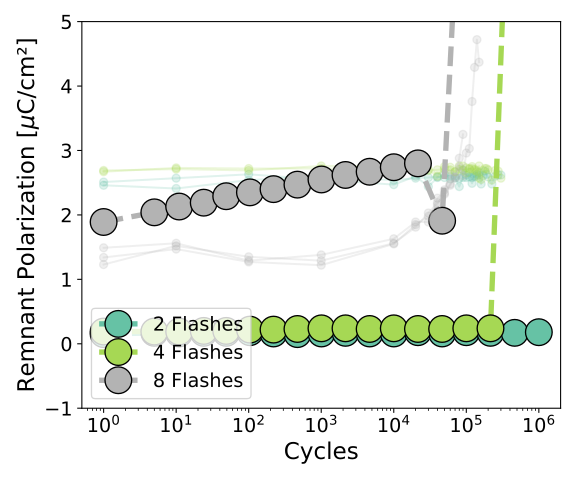
\includegraphics[width=.45\textwidth]{../Fig/FlashNumC_EnduTrends.png}
        (d)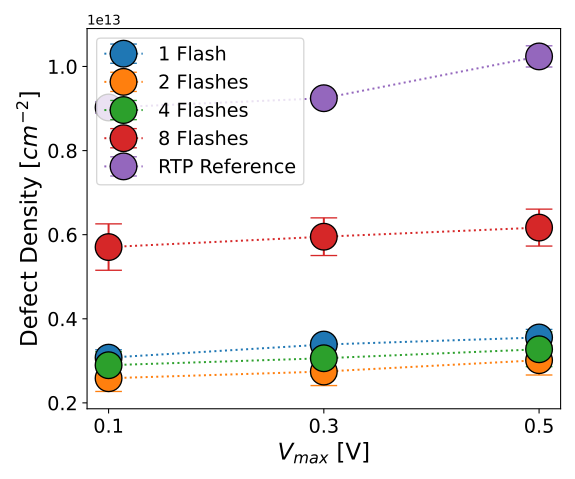
\includegraphics[width=.45\textwidth]{../Fig/FlashNumC_DDTrends.png}
        \caption{Figure showing Endurance and Defect Density from flashnumber-varied batches. Low-doped subtrate, 200C ALD, HZO 1:1, 250C preheat, 5ms flash at $\SI{20}{\joule/\centi\meter^2}$. RTP reference is included.}\label{fig:res_FlashNumAC_EnduDD}
    \end{figure}

    \begin{figure}[ht!]
        \centering
        (a)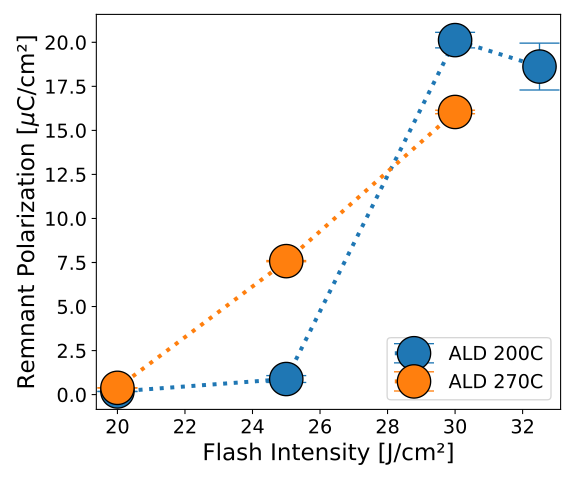
\includegraphics[width=.45\textwidth]{../Fig/FlashIntC+E_PrTrends.png}
        (b)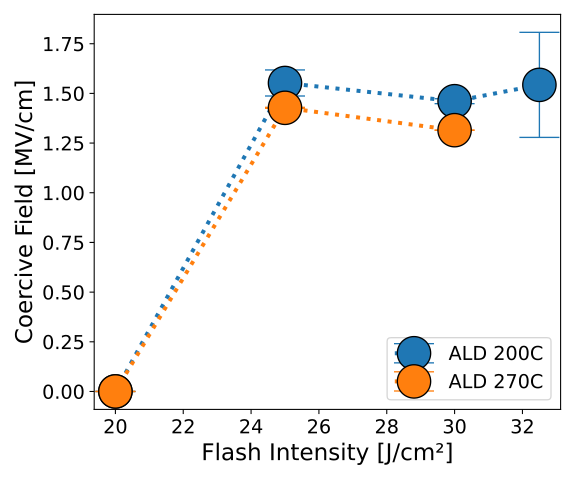
\includegraphics[width=.45\textwidth]{../Fig/FlashIntC+E_EcTrends.png}
        (c)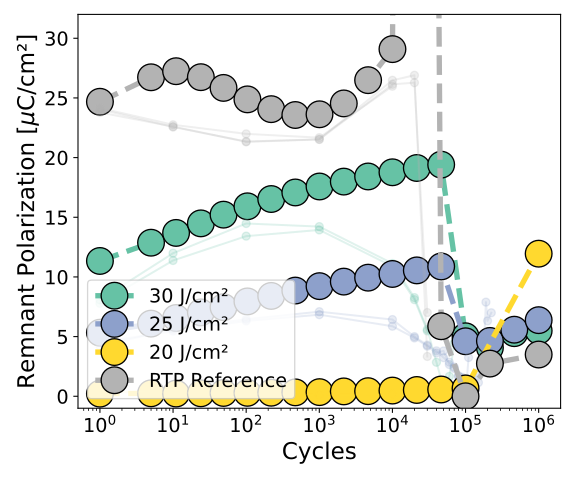
\includegraphics[width=.45\textwidth]{../Fig/FlashIntE_EnduTrends.png}
        (d)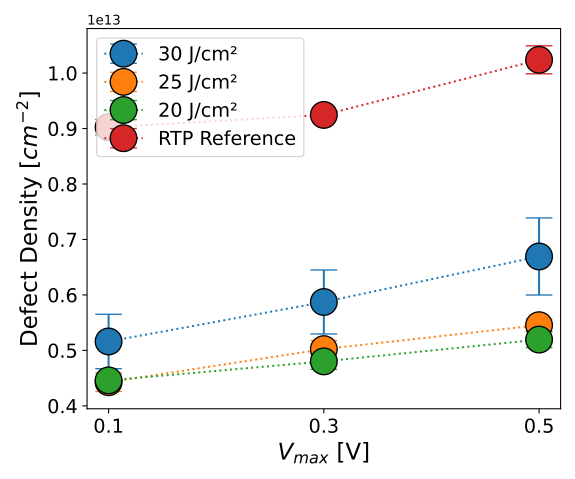
\includegraphics[width=.45\textwidth]{../Fig/FlashIntE_DDTrends.png}
        \caption{Figure showing all measured data from an intensity-varied batch. Low-doped subtrate, 270C ALD, HZO 1:1, 250C preheat, 5ms flash. RTP reference is included for Endurance and Defect Density.}\label{fig:res_FlashIntE}
    \end{figure}

    \begin{figure}[ht!]
        \centering
        (a)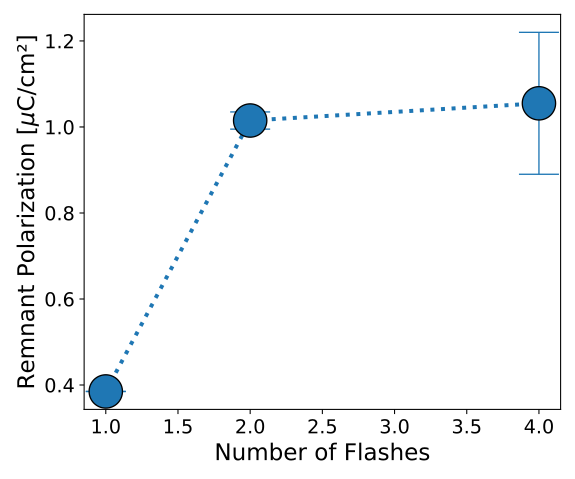
\includegraphics[width=.45\textwidth]{../Fig/FlashNumD_PrTrends.png}
        (b)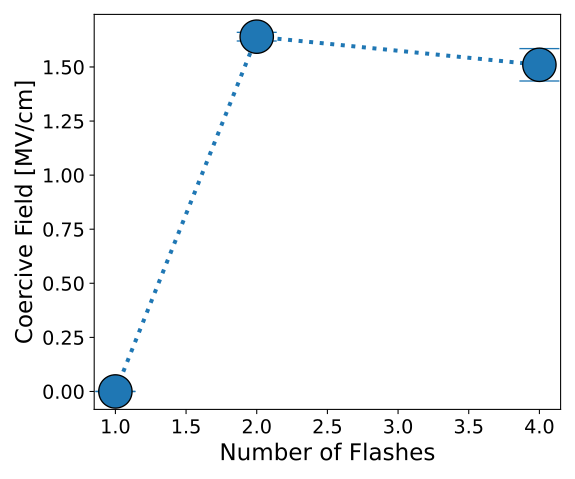
\includegraphics[width=.45\textwidth]{../Fig/FlashNumD_EcTrends.png}
        (c)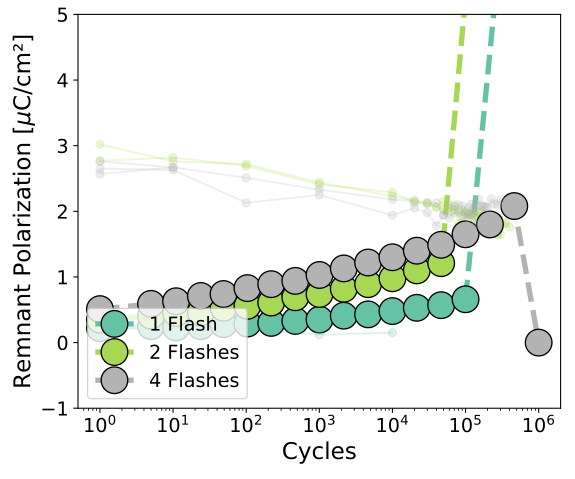
\includegraphics[width=.45\textwidth]{../Fig/FlashNumD_EnduTrends.png}
        (d)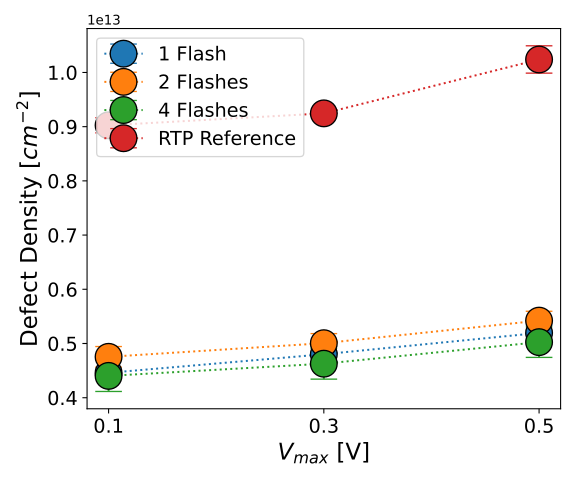
\includegraphics[width=.45\textwidth]{../Fig/FlashNumD_DDTrends.png}
        \caption{Figure showing all measured data from a flashnumber-varied batch. Low-doped subtrate, 270C ALD, HZO 1:1, 250C preheat, 5ms flash.}\label{fig:res_FlashNumD}
    \end{figure}

    \section{Conclusion}

    Mål: Wrap it up. Lägg fram de främsta resultaten/ideerna och ge tips på hur man kan undersöka vidare.

    \section{References}
        \bibliography{MasterThesis.bib}
        \bibliographystyle{ieeetr}

\end{document}
